%!TEX root=../document.tex

\section{Ergebnis}
\label{sec:Ergebnis}

Folgende Punkte wurden bearbeitet:

\begin{itemize}
	\item Überblick erhalten
	\item Installieren von CAS Server
	\item Ausführen des CAS Servers
	\item Https konfigurieren
\end{itemize}

\subsection{Überblick erhalten}

Zu beginnt der Übung habe ich noch immer nicht ganz verstanden, wie der CAS Server ausgeführt wird, ob das eine eigenständige Anwendung ist, ob das nur einen Erweiterung für eine Projekt ist, ob ich CAS an einen Dienst anhängen muss.
\newline
Zusätzlich habe ich dann ewig im Internet nach einem Quick-Start und einem erweitertem Tutorial gesucht. Ein Tutorial habe ich zwar gefunden, habe allerdings erst etwas spät bemerkt, dass dieses Tutorial seit über einem Jahr veraltet ist und nicht mehr verwendet werden sollte und hat mich auf die offizielle Webseite weitergeleitet. Etwas ähnliches wie einen Quick-Start habe ich nicht gefunden, daher hatte/habe ich noch immer einen klare Vorstellung, wie die Struktur auf dem Server und auf dem Client aussehen soll und über Technologie ich einsetzen soll, außer Tomcat und CAS.
\newline 
Zuletzt habe ich dann begriffen, dass der Server zumindest über eine war-Datei auf einem Tomcat Server deployed werden kann und damit den ersten Schritt legt.

\subsection{Installieren von CAS Server}

Als ersten Schritt habe ich den CAS Server heruntergeladen/installieren und dabei einige Möglichkeiten versucht.

\subsubsection{Installieren mittels source als zip}

Hierbei habe ich über den Link, welcher in der Aufgabebeschreibung bereitgestellt war, den cas server als Sourcecode für Java heruntergeladen. Darauf hin hab ich mir gedacht, dass die Sourcedateien in einem Java Projekt verwendet werden müssen. Allerdings fand ich keine Anleitung, wie ich die Sourcedateien im ein Java Projekt implementiere und dann deployen kann. Daher habe ich diesen Weg wieder verworfen.

\subsubsection{Installieren mittels vorkonfiguriertem Projekt}

Als zweite Option habe ich auf der offiziellen Webseite von CAS einen Link zu einer Webseite gefunden, die Eclipse Maven/Gradle Projekt modular zusammenbauen kann. Dort habe ich ein Maven Projekt ausgewählt und 'Tomcat' als Rolle hinzugefügt und dieses Projekt dann heruntergeladen. Dieses Projekt habe ich dann in Eclipse einfügt und dann hat er begonnen Abhängigkeiten herunterzuladen. Das hat allerdings kein Ende nach 10 Minuten genommen, also hab ich dieses Idee verworfen.

\subsubsection{Installieren mittels template}

Zuletzt habe ich auf der offiziellen Webseite einen Link zu einem Github Repo gefunden, in dem ein Beispielrepo bereitgestellt wurde und einen Anleitungen, wie CAS gebuildet und deployed werden kann. Dieses Repo habe ich dann runtergeladen und in Eclipse als Maven Projekt eingebunden. Das hat dann keine Probleme gemacht und konnte dann mit der Aufgabe weiter machen.

\subsection{Ausführen des CAS Server}

Nachdem ich ein Projekt mit einem CAS Server hatte, habe ich versucht diesen CAS Server auf einem Tomcat Server zu deployen.

\subsubsection{Ausführen über externe Konsole}

Als erstes habe ich, wie im Github Repo erklärt, die cas.war Datei über eine externe Konsole zu starten. Diese Methode gab mir ,neben einem Fehler, dass kein JAVA\_HOME Variable gefunden/richtig ausgeführt werden konnte, einen Fehler, dass der Prozess zu wenige Rechte hat, um den Server zu starten.

\subsubsection{Ausführen über integrierte Server von Eclipse}

Dann ist mir eingefallen, dass Eclipse eine Möglichkeit bittet, Tomcat Server über Eclipse zu starten. 
\newline
Davor musste ich aber noch alle Maven Probleme beseitigen, die mit dem Importieren entstanden sind. Also habe ich eine 'Maven Update' und eine 'Maven Build' mit Goal 'clean install' durchgeführt. Daraufhin habe ich eine neue Config für einen 'Apache Tomcat 9' Server erstellt und diesem das entsprechende Projekt zugewiesen.
\newline
Als ich den Server gestartet habe, bekam ich 2 unterschiedliche Fehler: 'Access Denied' und 'Failed to start child'.
\newline
Access Denied habe ich nur lösen können, indem ich die Serverkonfig/den Server in Eclipse komplett gelöscht und neu angelegt habe.
\newline
Failed to start child war meist einfach zu lösen, indem ich 'Maven Update' und 'Maven Build' mit Goal 'clean install' nochmals durchgeführt habe. Selten hat das nicht geholfen, da half auch nur noch gesamtes Projekt lösen und neu importieren.
\newline
Manchmal hat dann der Server mit CAS gestartet ohne Problem, abgesehen von dem Problem, dass Eclipse Server eigenständig terminiert, wenn diese nicht innerhalb von 45 Sekunden starten. Diese Einstellung habe ich bei jeder Serverkonfiguration jedesmal ändern müssen.

\begin{figure}[h]
\centering
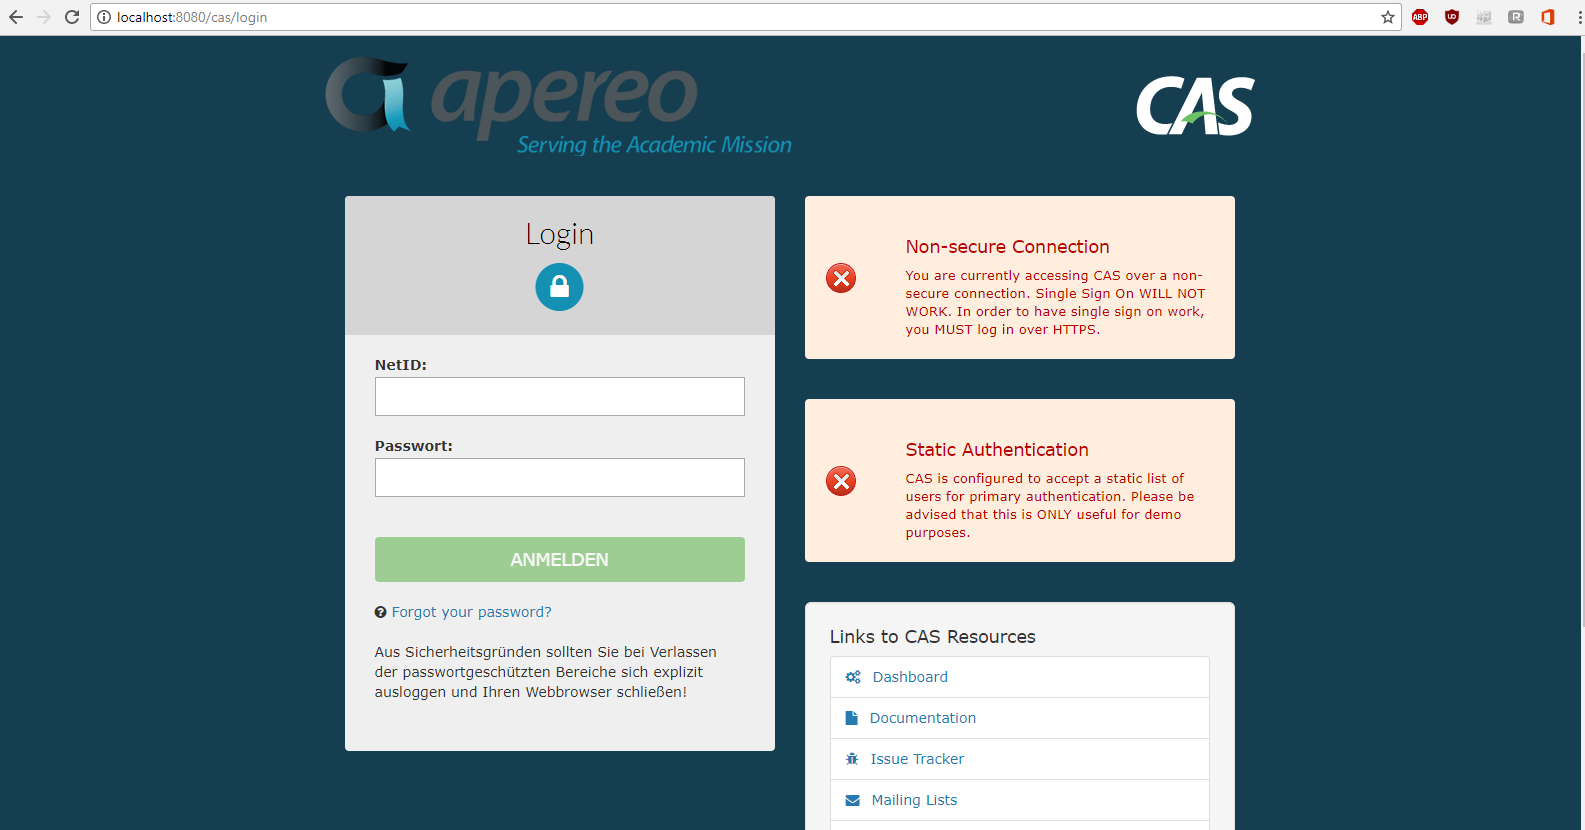
\includegraphics[width=0.7\linewidth]{images/bildCool}
\caption{Gestarteter CAS Server}
\label{fig:bildcool}
\end{figure}


\subsection{Https konfigurieren}

Als ich einen funktionierenden Server hatte, habe ich begonnen Https zu ermöglichen, da nur unter Https Single Log on funktioniert.
\newline
Als erstes habe ich mit dem Java-Tool keytool ein Zertifikat erstellt und dieses im Projektordner gespeichert.
\newline
Dann habe ich die Konfiguration des Tomcat Server gesucht und habe dort den SSL Connector eingeschaltet und angepasst.
\newline
Als ich dann versucht habe, den Server zu starten und dann startet der Server nicht mehr mit dem Felher Access Denied.
